

\section{Тестирование на гармоническом осцилляторе}
Дабы отбросить все сомнения в корректности работы программы для решения задачи Коши, проведём тестирование на более простом случае с заранее известным решением, а именно на гармоническом осцилляторе
\[
\begin{cases}
	\frac{d x}{d t} = y;\\
	\frac{d y}{d t} = -x;\\
	0 < t < 30; \\
	t = 0: x = 0, y = 8.
\end{cases}
\]

Визуализация численного решения данной задачи с помощью нашей программы представлена в виде графиков на рис.(\ref{t-x}), (\ref{t-y}) и (\ref{x-y}). Для удобства проверки дополнительно решим нашу задачу с помощью пакета {\it Wolfram Mathematica 9} (см.~рис.~\ref{Wolfram}).
Сравнивая полученные результаты можно заметить, что полученные решения абсолютно идентичны, на основе чего можно сделать вывод о корректности работы программы. Однако, для большей достоверности проверим так же численные оценки отклонений.\\
\begin{enumerate}
\item 
Для вычисления глобальной погрешности введём множество переменных $\delta_i:$ 
\[
 \delta_0 = 0, \qquad \delta_{k+1} = Err_{k} + \delta_{k} \cdot e^{\int\limits_{t_k}^{t_{k+1}} \mu(s) ds} 
\]
Интеграл в предыдущем выражении можно приблизить следующим образом
\[
\int\limits_{t_k}^{t_{k+1}} \mu(s) ds = (t_{k+1} - t_k) \cdot \mathrm{Hmax} \left(\frac{J + J^T}{2} \right),
\]
где $J$ "--- матрица Якоби исходной системы дифференциальных уравнений,  $Err_k$ "--- максимум расстояний между соответствующими координатами на $k$-ом шаге, а $\mathrm{Hmax}$ "--- функция, возвращающая максимальное собственное значение полученной матрицы. 
В наше случае мы получим следующее
\[
J = \left(
\begin{array}{cc}
 0 & 1 \\
 -1 & 0 \\
\end{array}
\right),
\qquad
A = \frac{J + J^T}{2} =
\left(
\begin{array}{cc}
 0 & 0 \\
 0 & 0 \\
\end{array}
\right)
\]
\[
\lambda_{1,2} = 0, \qquad \delta_0 = 0, \qquad \delta_{k+1} = Err_{k} + \delta_{k}.
\]
Таким образом были получены следюущие значения глобальной погрешности:
\[
\text{для точности погрешности -7-го порядка } \delta_k =  2.433796 \cdot 10^{-6}
\]
\[
\text{для точности погрешности -9-го порядка } \delta_k =  3.964618 \cdot 10^{-7}
\]
\[
\text{для точности погрешности -11-го порядка } \delta_k =  8.135620 \cdot 10^{-9}
\]

\item А оценка {\bf локального отклонения на шаге} для каждой точки $t = \{50, 100, 150, 200\}$ для обеих координат получилась равна в районе $100 \pm 2$, что намного превышает теоретическую оценку 56.23 и свидетельствуют о~большом запасе точности в методе "--- при уменьшении максимально допустимой относительной погрешности на шаге интегрирования на 2 порядка происходит существенное уточнение решения, метод в~данном случае работает как метод более высокого порядка. Это в первую очередь связано с коэффициентами в~расчётных формулах метода и особенностями системы дифференциальных уравнений гармонического осциллятора.
\end{enumerate}

На основе выше сказанного можно сделать вывод, что полученная программа работает корректно.
\newpage
\begin{figure}[H]
\centering
    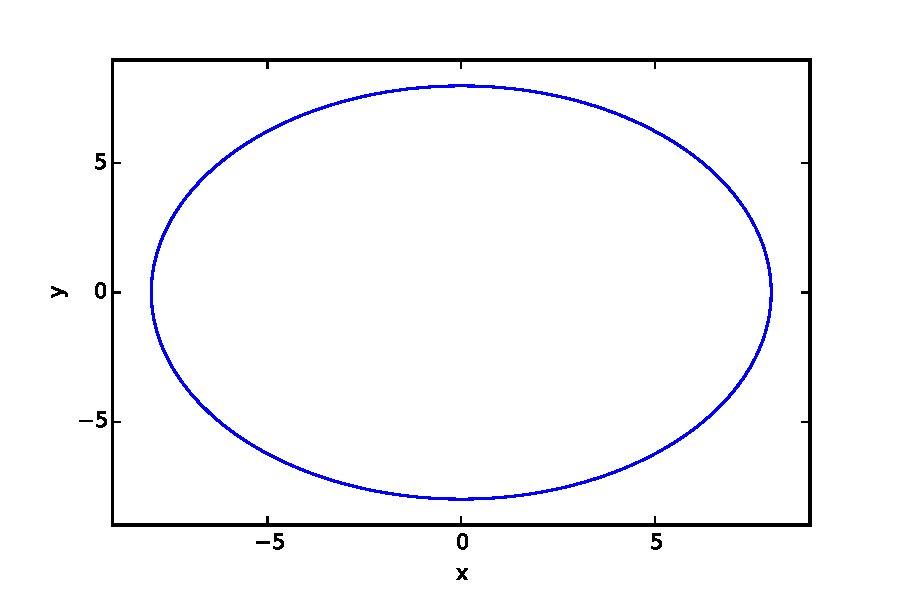
\includegraphics[width=100mm]{pictures/x-y.pdf}
    \caption{Решение задачи о математическом осцилляторе. График зависимости $y(x)$}
    \label{x-y}
\end{figure}
\begin{figure}[H]
\centering
    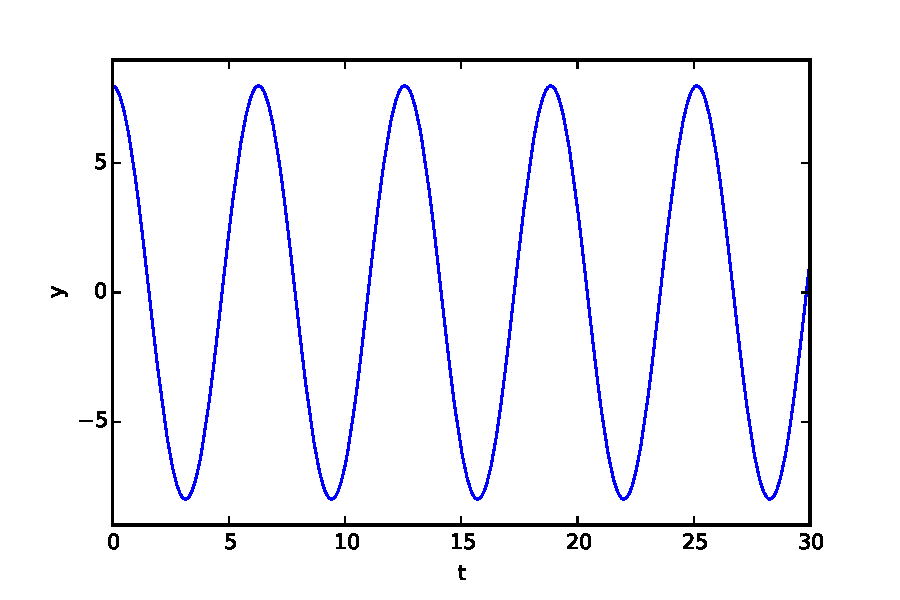
\includegraphics[width=100mm]{pictures/t-y.pdf}
    \caption{Решение задачи о математическом осцилляторе. График зависимости $y(t)$}
    \label{t-y} 
\end{figure}
\begin{figure}[H]
\centering
    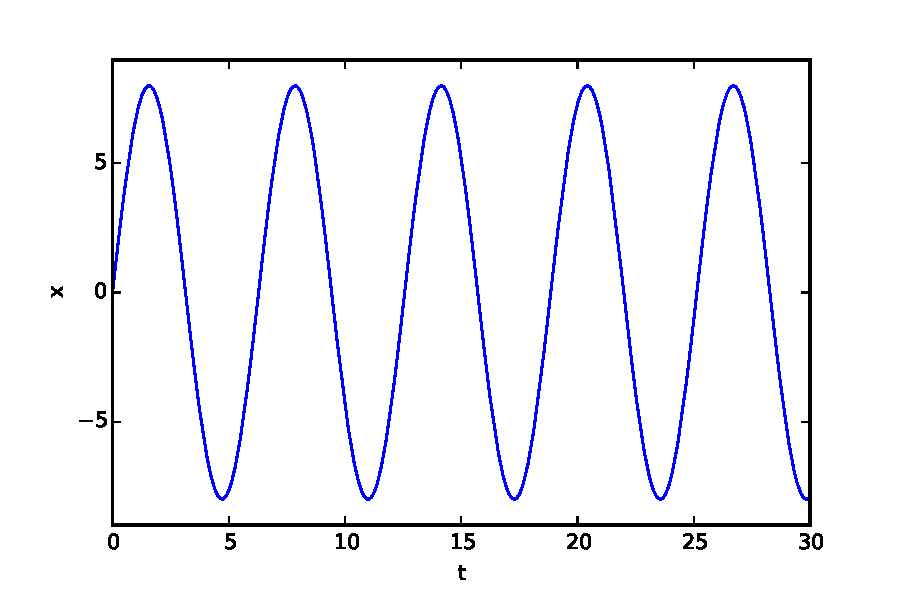
\includegraphics[width=100mm]{pictures/t-x.pdf}
    \caption{Решение задачи о математическом осцилляторе. График зависимости $x(t)$}
    \label{t-x}
\end{figure}
